
\section{Introduction}



\begin{frame}{Introduction}
    \framesubtitle{Verification of a Document}

Organizations issue documents to certify that a specific fact has occurred.\\
These documents may be physical or digital.\\
\vspace*{0.2cm}
In current practice, document verification is usually performed by the issuing organization itself.\\
\vspace*{0.2cm}
This verification requires checking three fundamental properties:
\vspace*{0.2cm}
\begin{itemize}
    \item The content has not been altered.
    \item The document was issued by the claimed organization.
    \item The document has not been revoked.
\end{itemize}
\end{frame}


\begin{frame}
\begin{block}{Example: Academic Certificate}
\vspace*{0.2cm}
An academic certificate illustrates the requirements of document verification:
\vspace*{0.2cm}
\begin{itemize}
    \item Integrity: The content (names, dates, degree) must not be modified.
    \item Authenticity: The certificate must be issued by the legitimate institution.
    \item Validity: The certificate may become invalid if revoked due to error or fraud.
\end{itemize}
\end{block}
\end{frame}


\begin{frame}{Introduction}
\framesubtitle{Verification Problem}
\definecolor{CustomBlue}{HTML}{0072B2} 
\setbeamercolor{block title}{fg=white, bg=CustomBlue}
\begin{block}{Remark}
“The global market for certificate forgery and fraud is estimated to exceed two trillion USD annually.”~\cite{Xie2020EthereumCertificate}
\end{block}

Document forgery directly undermines trust in issuing institutions.\\
\vspace*{0.2cm}
In traditional physical systems, document verification is centralized and requires significant operational resources, including personnel, infrastructure, and anti-tampering measures.\\
\vspace*{0.2cm}
In digital systems, verification remains centralized and introduces additional costs related to service availability, Denial-of-Service protection and server-side cybersecurity.
\end{frame}



\begin{frame}{Introduction}
\framesubtitle{Decentralized Networks}
\begin{columns}[T]  
\column{0.5\textwidth}
Bitcoin is the first decentralized network, operating continuously since January 3, 2009.\\
It is secured by a \textbf{Proof of Work (PoW)} consensus protocol and elliptic-curve cryptography.
\column{0.5\textwidth}
\vspace*{0.25cm}
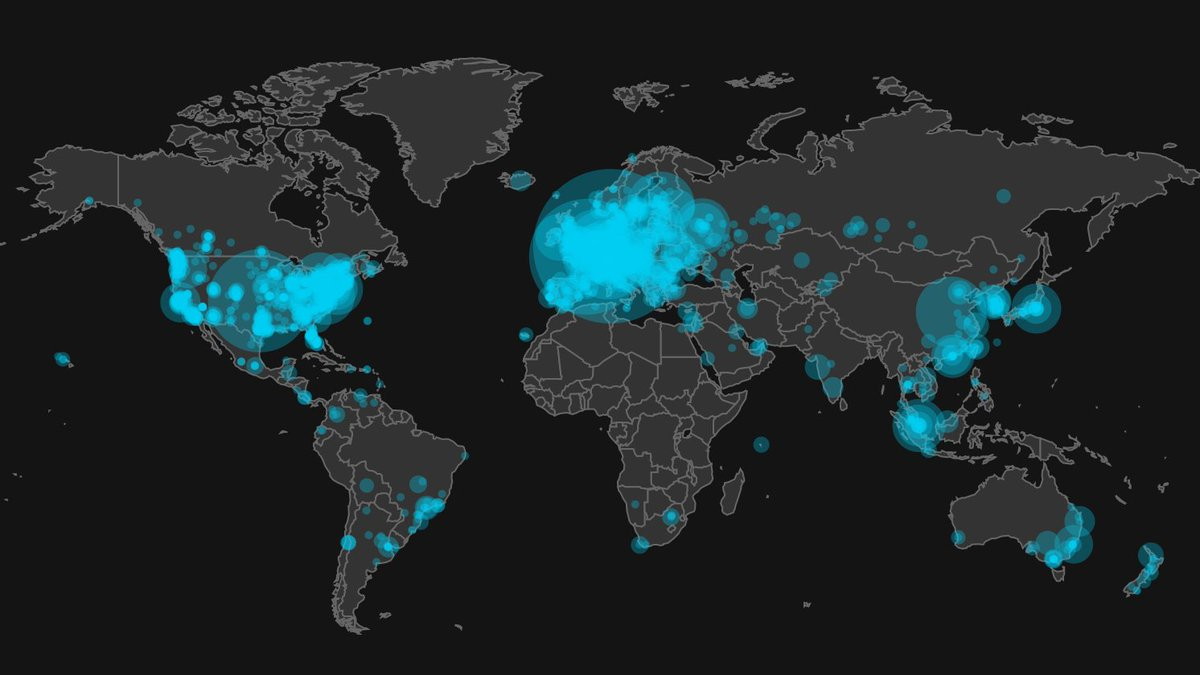
\includegraphics[scale=0.1]{figures/nodes.jpg}
\end{columns}
\vspace*{0.3cm}
Its main properties are:
\vspace*{0.1cm}
\begin{itemize}
\item Censorship resistance and permissionless participation
\item High availability through global replication.
\item An immutable public ledger.
\item Public verifiability without trusted intermediaries.
\end{itemize}

\end{frame}



\begin{frame}{Introduction}
    \framesubtitle{Why Bitcoin? 
\includegraphics[scale=0.0065]{figures/bitcoin.png}}
Bitcoin is designed to minimize the attack surface of the network.\\
Reduces the risk of Denial-of-Service (DoS) attacks by limiting on-chain computation.\\

\vspace{0.2cm}
This is achieved through:
\begin{itemize}
    \item Stack programming language.
    \item A small and fixed set of opcodes (e.g., arithmetic, comparison, signature checks).
    \item Does not allow recursion, loops, or persistent memory.
\end{itemize}
Using the Unspent Transaction Output UTXO model, each transaction is independent.
\end{frame}



\begin{frame}{Introduction}
\framesubtitle{Blockchain Networks with complex smart contracts}
Other blockchain platforms, such as Ethereum, adopt an account-based model instead of UTXO.\\
\vspace{0.2cm}
They execute programs on the Ethereum Virtual Machine (EVM), enabling expressive logic with loops, recursion, and access memory.
\vspace*{0.2cm}
\begin{block}{\textbf{The Trade-off}}

Increased expressiveness comes at the cost of higher execution fees, greater system complexity, and a larger attack surface compared to Bitcoin’s constrained execution model.
\end{block}
\end{frame}


\begin{frame}{Introduction}
\framesubtitle{Decentralized Networks for Document Verification}

Decentralized blockchain networks enable new models for digital document verification.\\
Instead of relying on a single organization to validate documents, verification can be performed independently using public blockchain data.\\
\vspace{0.2cm}
For document verification, this model provides:
\begin{itemize}
    \item High availability without dependence on centralized infrastructure.
    \item Resistance to denial-of-service and censorship attacks.
    \item Immutable records that preserve data integrity over time.
    \item Cryptographic proofs that prevent repudiation by the issuer
\end{itemize}

\end{frame}